\section{Validation}
\label{sec:validation}

\begin{figure}[]
\centering
       \subfigure[Line Network, $I_S = 18 KB$]{
        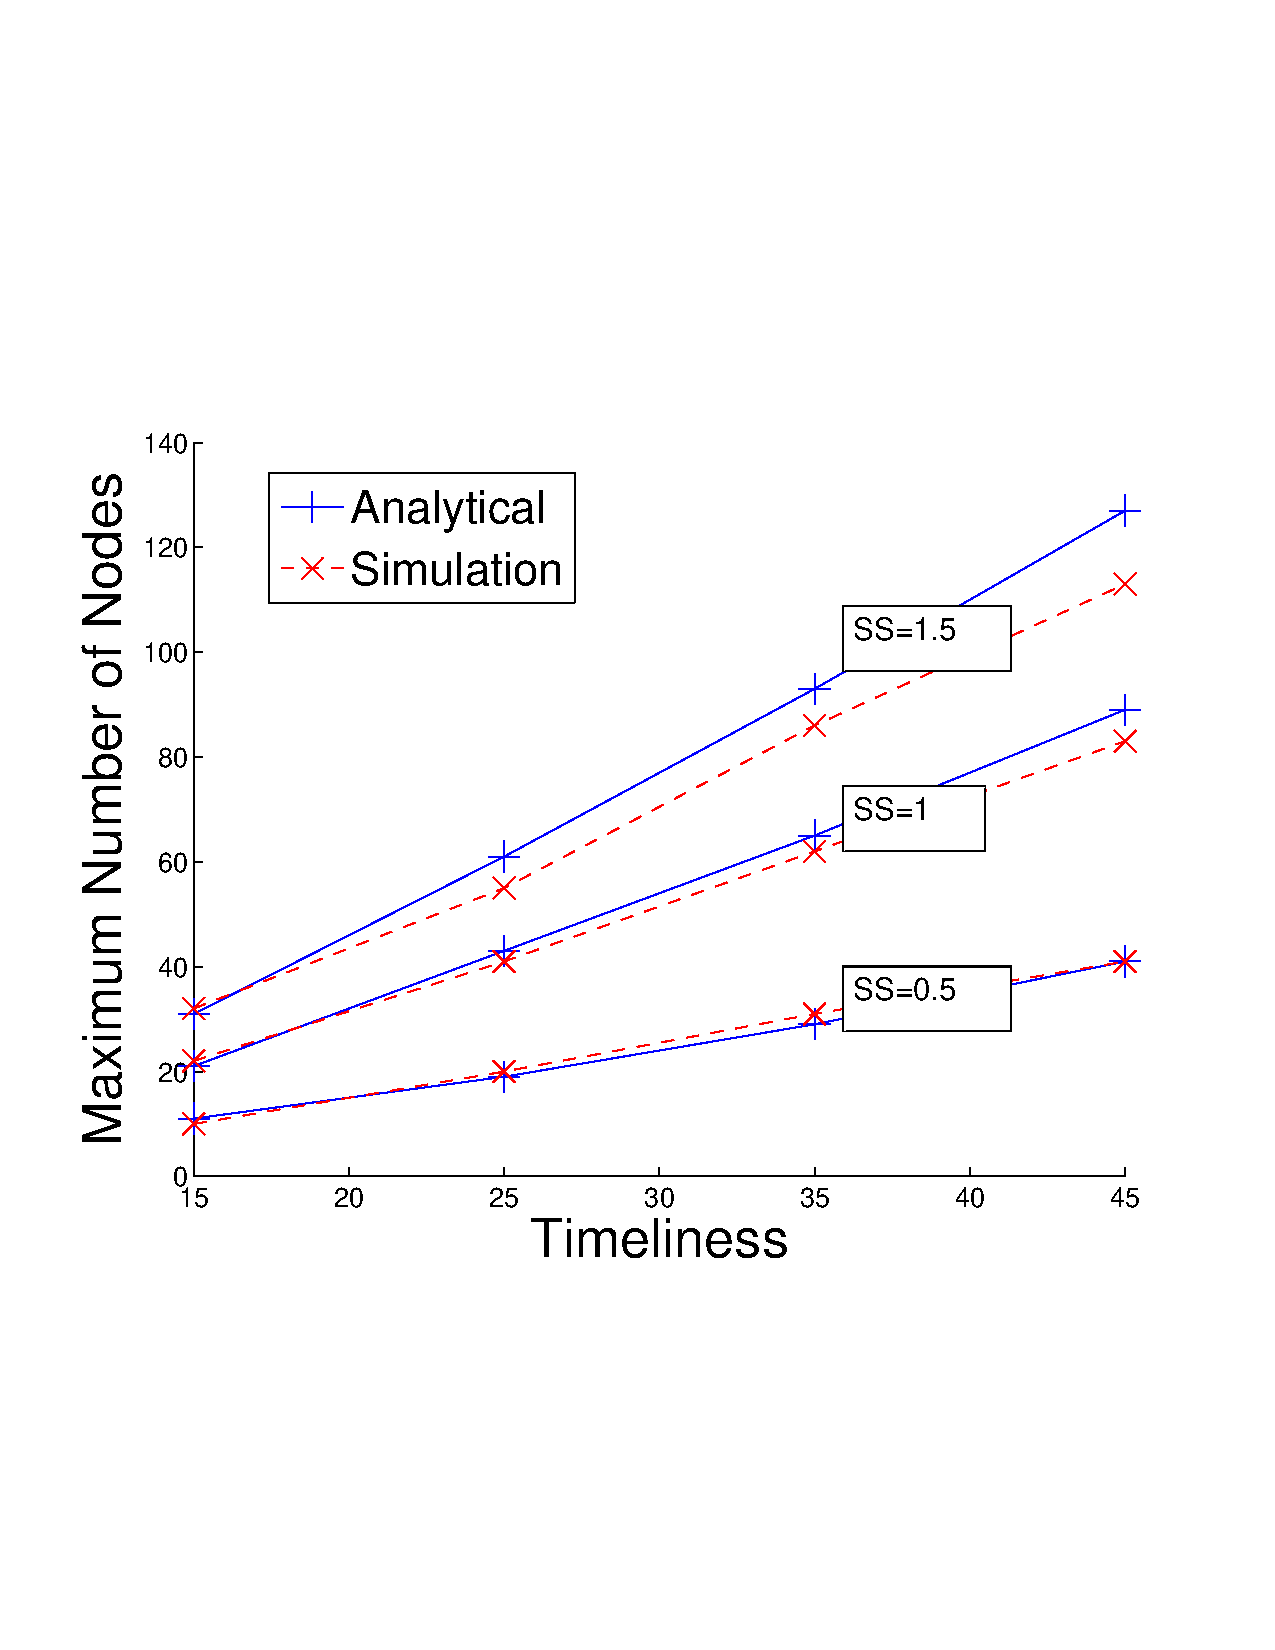
\includegraphics[scale=0.40, clip=true, trim=12mm 65mm 20mm 65mm]{figures/scal_sim_results/line_scal_anal_vs_sim_color.pdf}
        \label{fig:scal_vs_qoi_line}
        }
    \subfigure[Grid Network, $I_S = 48 KB$]{
        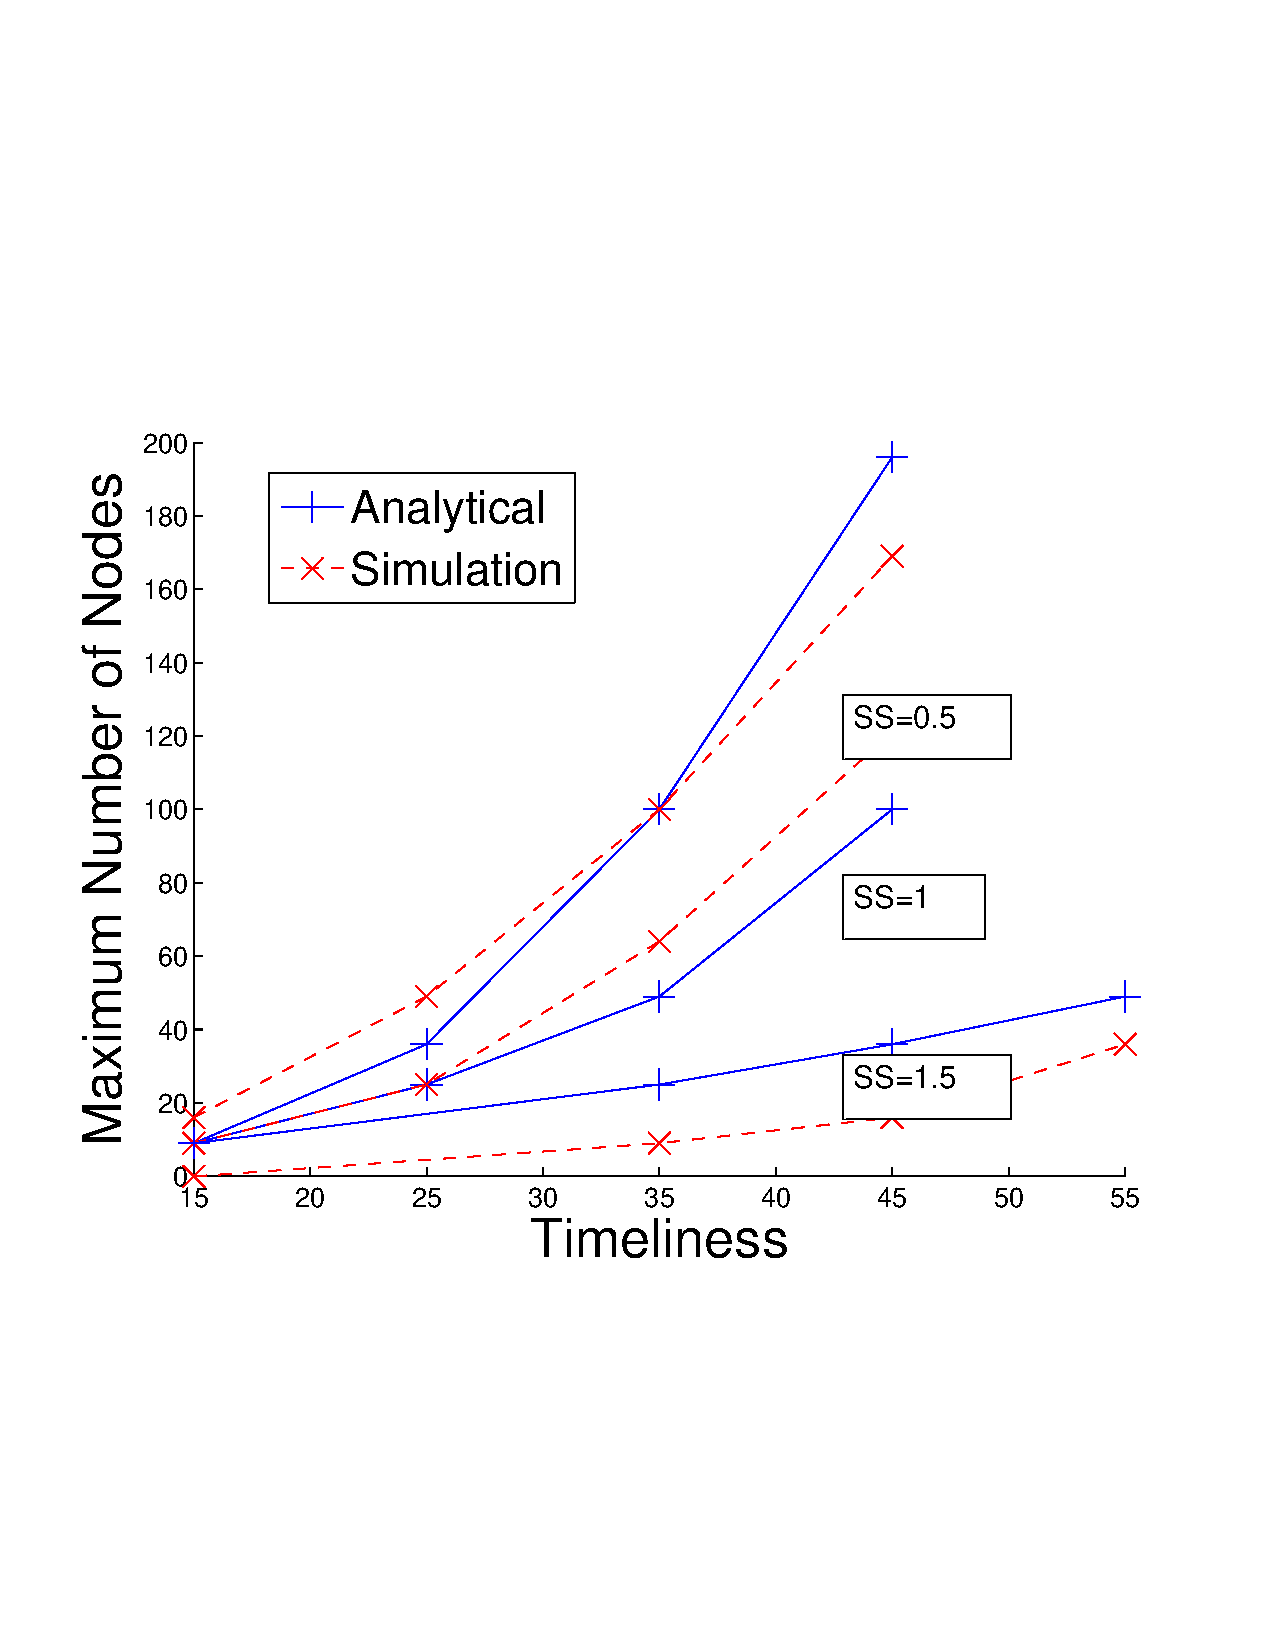
\includegraphics[scale=0.40, clip=true, trim=12mm 65mm 20mm 65mm]{figures/scal_sim_results/grid_scal_anal_vs_sim_color.pdf}
        \label{fig:scal_vs_qoi_grid}
        }
   \caption{Empirical results match analytical results closely for all tests.}
   \label{fig:scal_vs_qoi}
\end{figure}

To show how effective estimates using this framework can be, we simulated the network topologies and traffic described above in Section \ref{sec:example_applications} in the ns3 network simulator, comparing empirical results to those generated analytically with this framework, labeled \emph{Analytical}.  
%Due to space concerns, we only show a subset of results in Figure \ref{fig:scal_vs_qoi} to provide evidence of the effectiveness of the methodology.  All results generated, however, exhibit very similar trends of proximity between empirical and the analytical values.
We use a channel rate of $W= 2 Mbps$, packet sizes of $P_s = 1500$ bytes, and image sizes of $36$ and $72$ Kbytes.  As above, the correlation between Sum Similarity and $k_{req}$ is taken from the actual observed relation in Figure \ref{fig:topkSumSim}.  All values of parameters ($SS$, $T$, $I_S$, etc.) were chosen to test a variety of network sizes and QoI requirements while remaining within realistic network sizes, both with respect to real-world deployments and simulations with feasible run-times.

%Figure \ref{fig:scal_vs_qoi} shows the maximum scalability projected by solving inequalities (\ref{eq:clique_gen})-(\ref{eq:grid_gen}) and the maximum scalability observed in our experiments.  In our simulations, we defined \emph{scalable} as a network in which all of the requested queries were entirely fulfilled within the specified timeliness requirement.  Small differences arise due to average values being used for $CF$, $TF$, $DF$, and $PL$, but, as the graphs show, in all of these scenarios, our network size estimates are very close to those realized in practical simulations.


%\begin{figure*}[]
%\centering
%    \subfigure[Clique Network, $I_S = 9 MB$]{
%        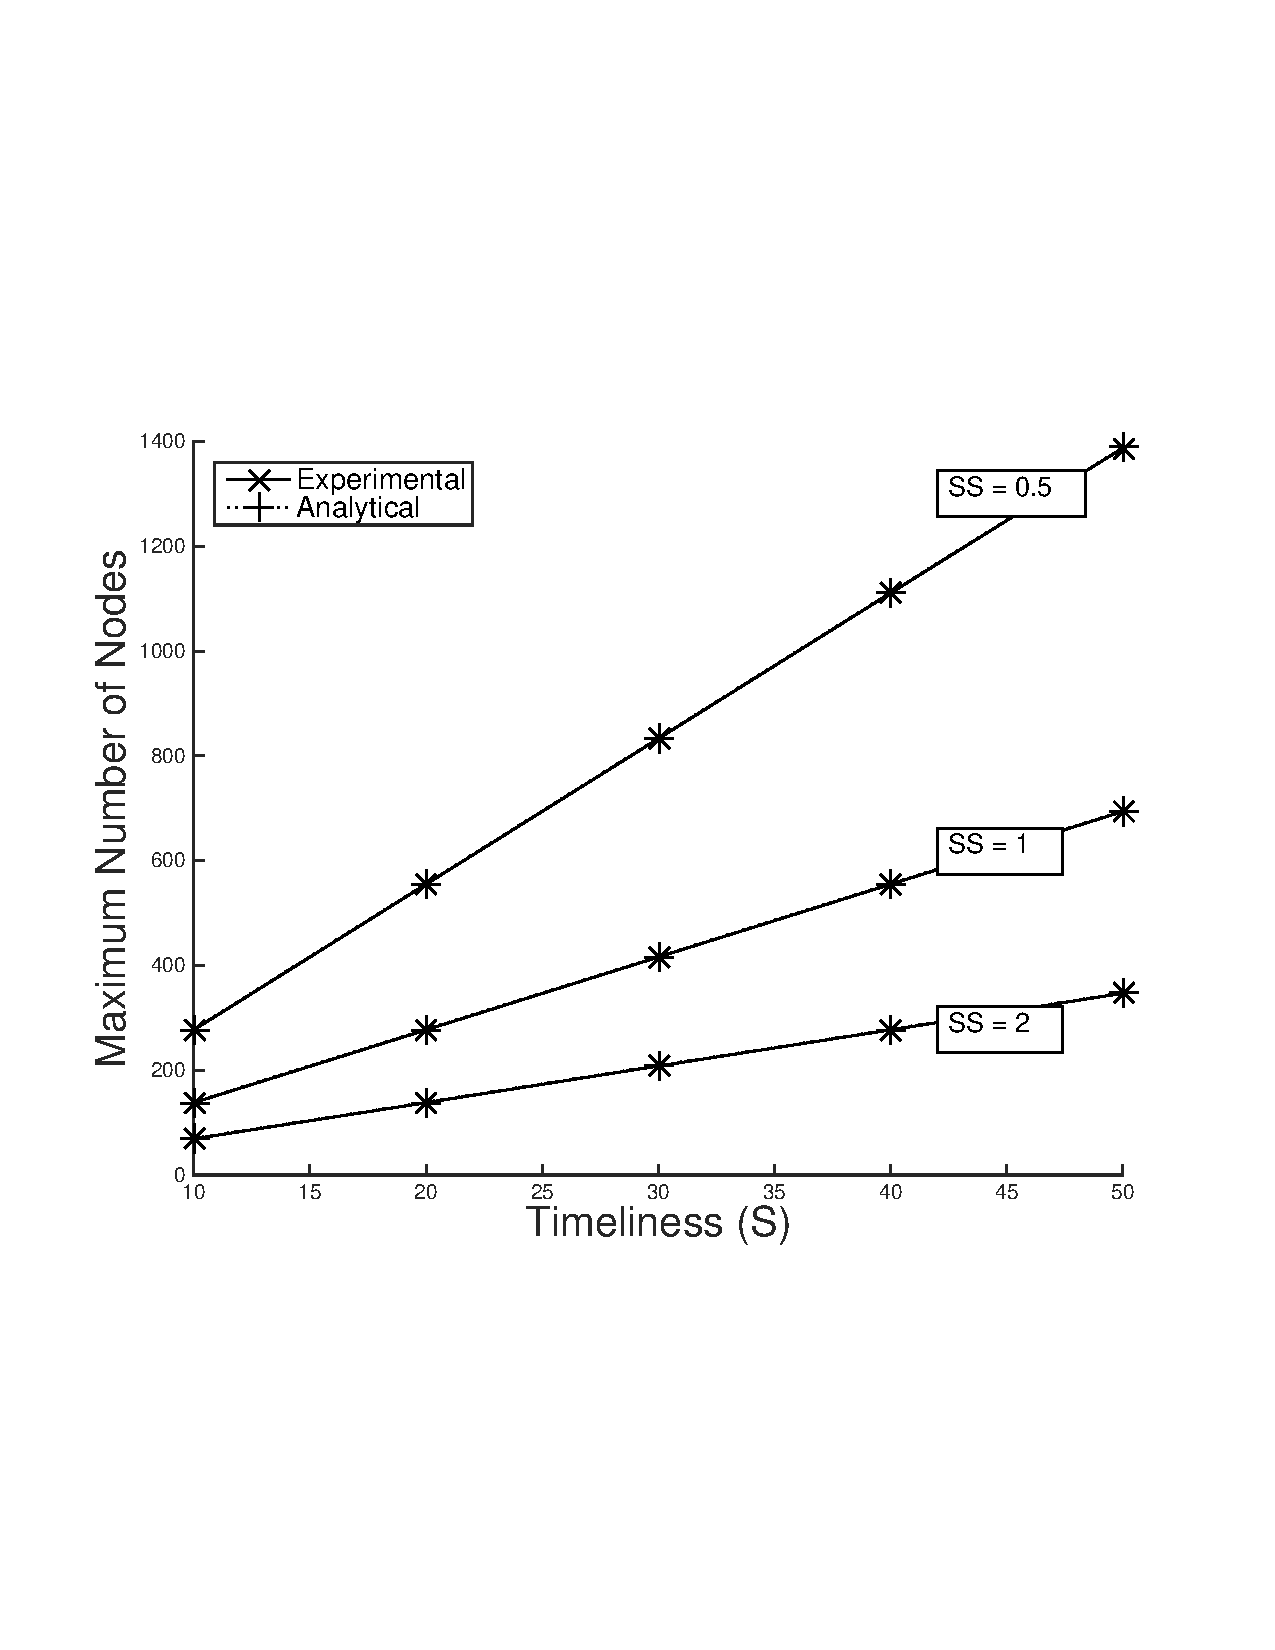
\includegraphics[scale=0.29, clip=true, trim=15mm 65mm 20mm 65mm]{figures/scal_sim_results/clique_uni_2d.pdf}
%        \label{fig:scal_vs_qoi_clique}
%        }
%    \subfigure[Line Network, $I_S = 12 MB$]{
%        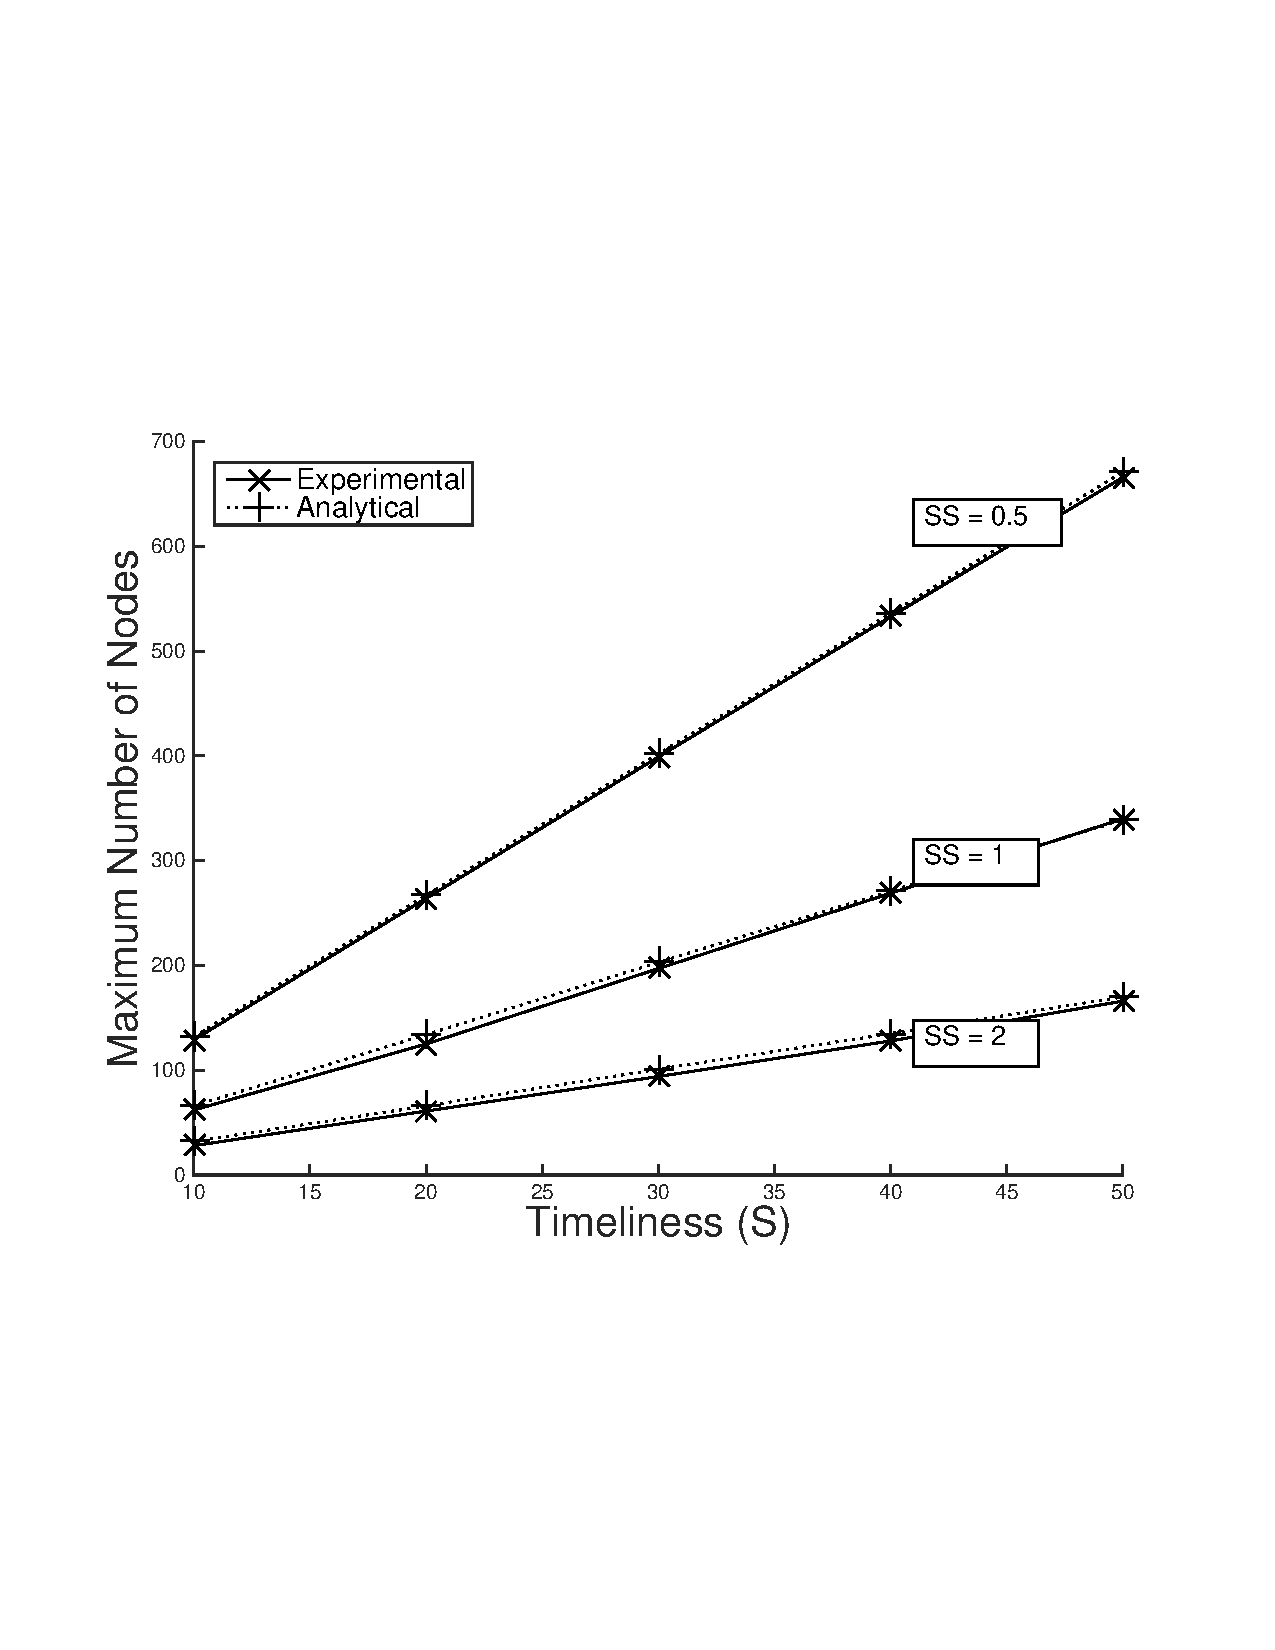
\includegraphics[scale=0.29, clip=true, trim=15mm 65mm 20mm 65mm]{figures/scal_sim_results/line_uni_2d_mhop_2.pdf}
%        \label{fig:scal_vs_qoi_line}
%        }
%    \subfigure[Grid Network, $I_S = 48 MB$]{
%        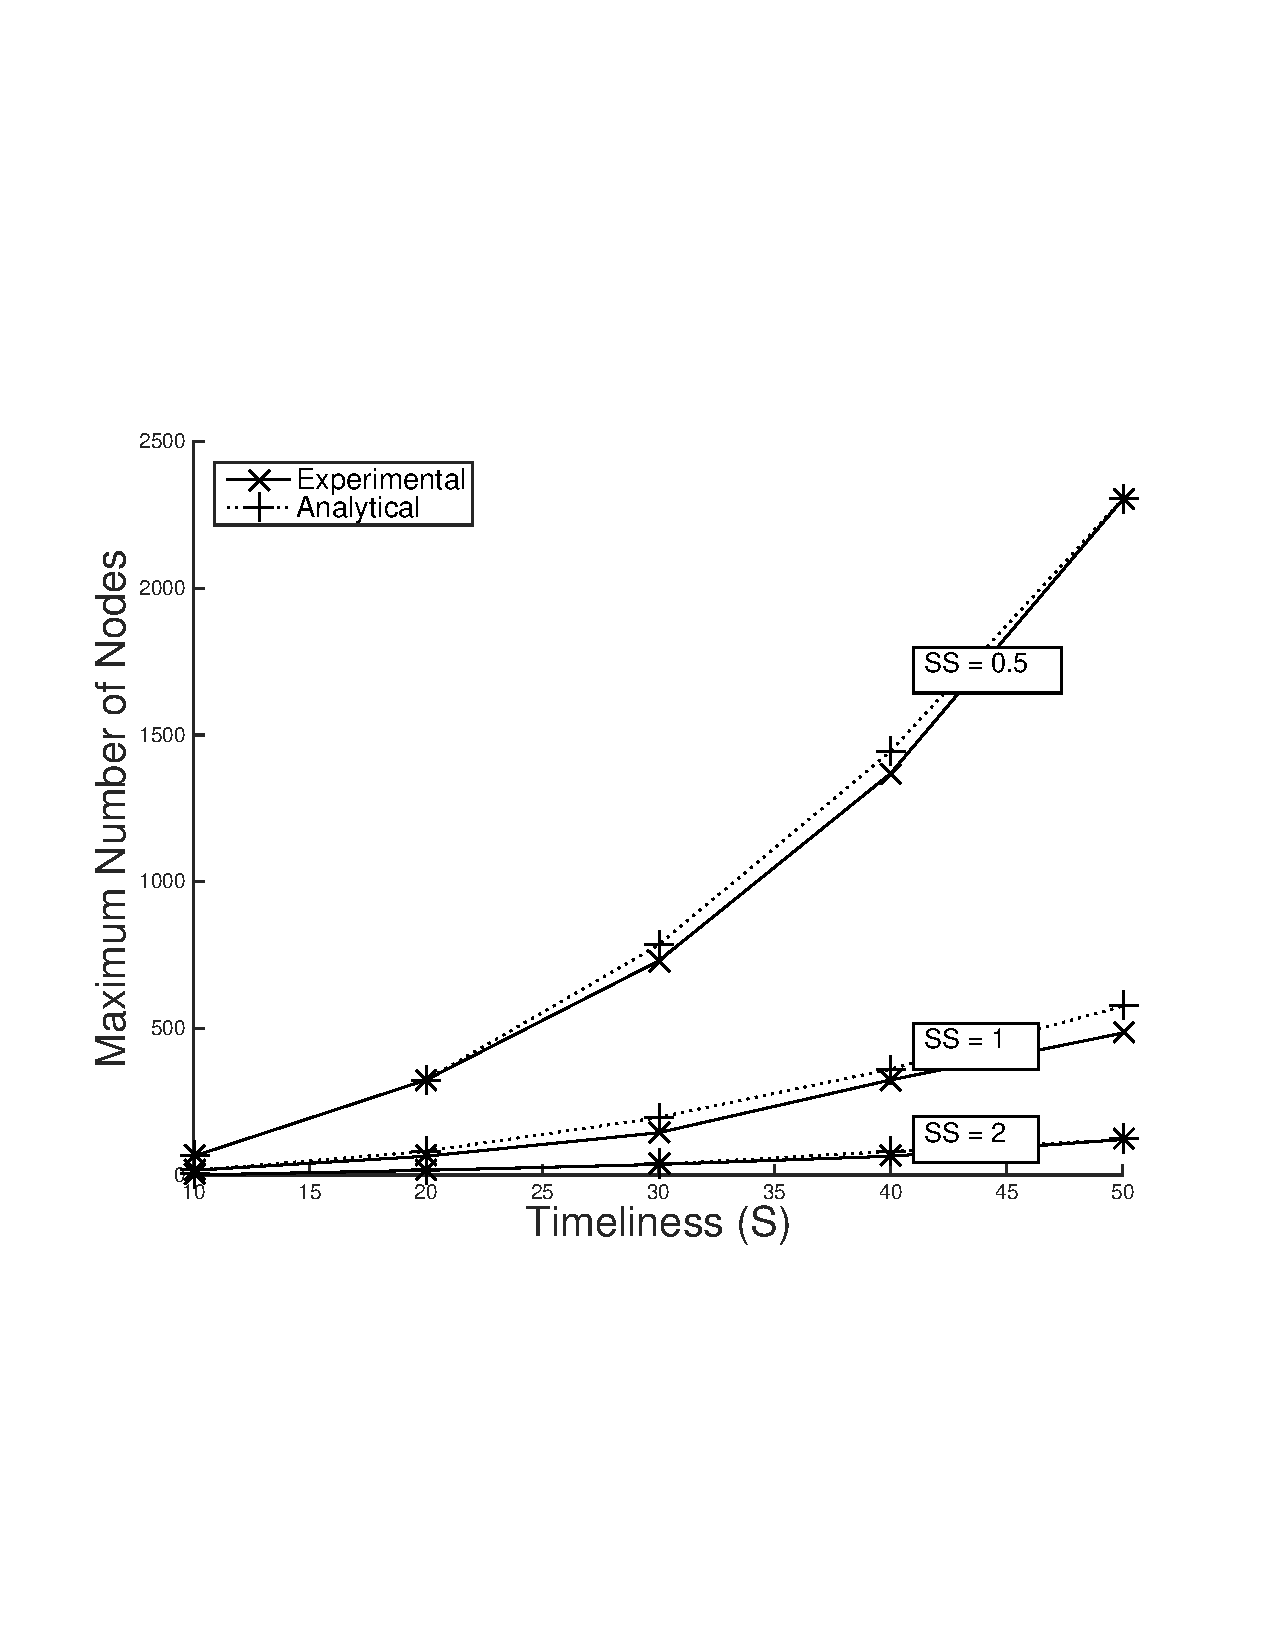
\includegraphics[scale=0.29, clip=true, trim=15mm 65mm 20mm 65mm]{figures/scal_sim_results/grid_uni_2d_mhop_2.pdf}
%        \label{fig:scal_vs_qoi_grid}
%        }
%   \caption{Empirical results match analytical results closely for all performed tests.  Results for each topology and a variety of sum similarity (SS) and timeliness requirements are provided.}
%   \label{fig:scal_vs_qoi}
%\vspace{-6mm}
%\end{figure*}
